% presentation.tex
% Matthew Monaco
% Andy Sayler
% Landon Spear

\documentclass[xcolor=dvipsnames]{beamer}
\usetheme{AnnArbor}
\usecolortheme{beaver}
\setbeamercovered{transparent=25}
\setbeamertemplate{blocks}[rounded][shadow=false] 
\setbeamertemplate{navigation symbols}{}

\usepackage{graphicx}
\usepackage{url}
\usepackage{listings}

\bibliographystyle{plain}

\lstloadlanguages{C}
\lstset{
  language=C,
  basicstyle=\footnotesize,
  numbers=none,
  numberstyle=\footnotesize,
  stepnumber=1,
  numbersep=5pt,
  showspaces=false,
  showstringspaces=false,
  showtabs=false,
  tabsize=4,
  captionpos=b,
  breaklines=true,
  breakatwhitespace=false,
  title=\lstname,
  frame=single,
  frameround=tttt
}

\newenvironment{packed_enum}{
\begin{enumerate}
  \setlength{\itemsep}{1pt}
  \setlength{\parskip}{0pt}
  \setlength{\parsep}{0pt}
}{\end{enumerate}}

\newenvironment{packed_item}{
\begin{itemize}
  \setlength{\itemsep}{1pt}
  \setlength{\parskip}{0pt}
  \setlength{\parsep}{0pt}
}{\end{itemize}}

\title[NCD]{Networked Character Devices}
%\subtitle[]{}
\author[Monaco, Sayler, Spear]{Matthew Monaco \&
                               Andrew Sayler \&
                               Landon Spear}
\institute[CU-Boulder]{
  University of Colorado at Boulder \\
  \texttt{\{first.last\}@colorado.edu}
}
\date[Dec. 10, 2011]{Saturday, December 10\textsuperscript{th}, 2011}

\begin{document}

%---Title Slide---%
\begin{frame}[plain]
  \titlepage
\end{frame}

\begin{frame}{Outline}
  \tableofcontents
\end{frame}

%Landon - Beginning

\section{Overview}
%---Intro Slide---%
\begin{frame}{\bf NCD Overview}
  We did some stuff, we used some references \cite{ldd3}.
\end{frame}

\section{Introduction}

\section{Related Work}

% Matt - Middle

% Combine Architecture and System?
\section{Architecture}

\begin{frame}[c]{Very High Level}
  \begin{center}
    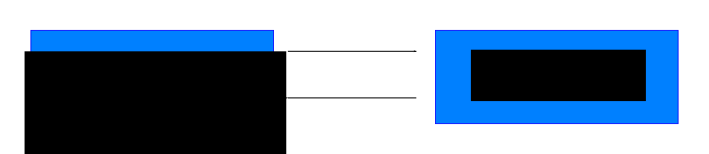
\includegraphics[width=0.8\textwidth]{arch-01.png}
  \end{center}

  \begin{itemize}
    \item<1-> Our system uses a basic client server model
    \item<2-> The client initiates all exchanges, the server replies
  \end{itemize}
\end{frame}

\begin{frame}[c]{High Level}
  \begin{center}
    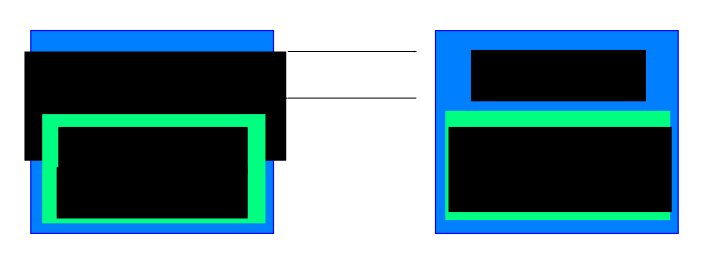
\includegraphics[width=0.8\textwidth]{arch-02.png}
  \end{center}

  \begin{itemize}
    \item<1-> The server side resides entirely in a single kernel module
    \item<2-> The client side is a standard userspace server
  \end{itemize}
\end{frame}

\begin{frame}[c]{Client Medium Level}
  \begin{center}
    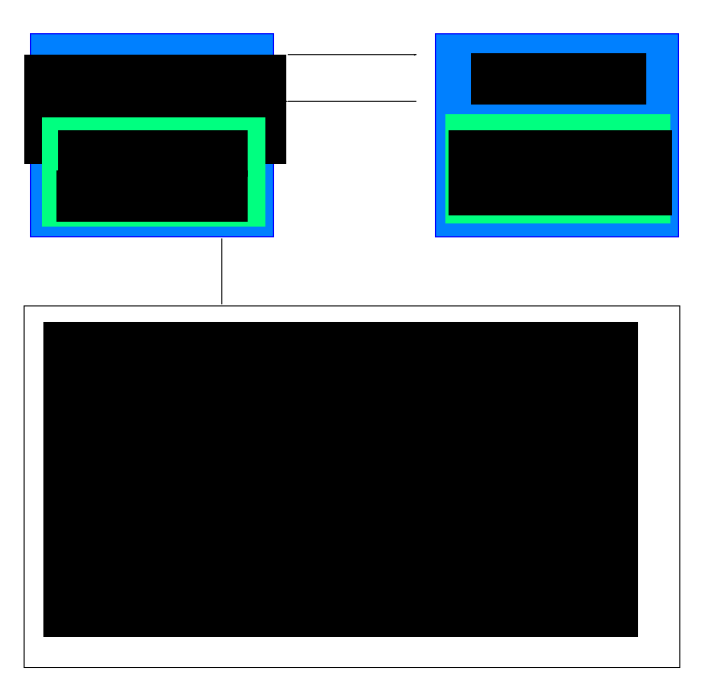
\includegraphics[width=0.4\textwidth]{arch-03.png}
  \end{center}

  \begin{itemize}
    \item<1-> By default, devices are exposed under /dev/netchar
    \item<2-> In the future, we should be able to choose any name
  \end{itemize}
\end{frame}

\begin{frame}[c]{Server Medium Level}
  \begin{center}
    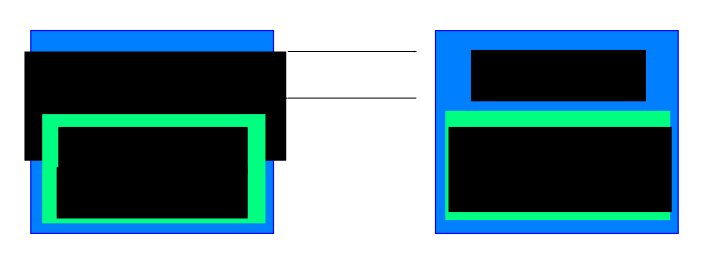
\includegraphics[width=0.8\textwidth]{arch-02.png}
  \end{center}
  \begin{itemize}
    \item<1-> Listen on a specified port
    \item<2-> Receive requests from client
    \begin{itemize}
      \item<2-> open,close,read,write,...
    \end{itemize}
    \item<3-> Can actually export \textit{any} file
    \item<4-> Crashes ungracefully when the client disconnects
  \end{itemize}
\end{frame}

\section{Implementation}

% Matt - End

% Andy Sections

\section{Results and Evaluation}
%---Full State Slide---%

\begin{frame}[c]{Full System}
  \begin{center}
    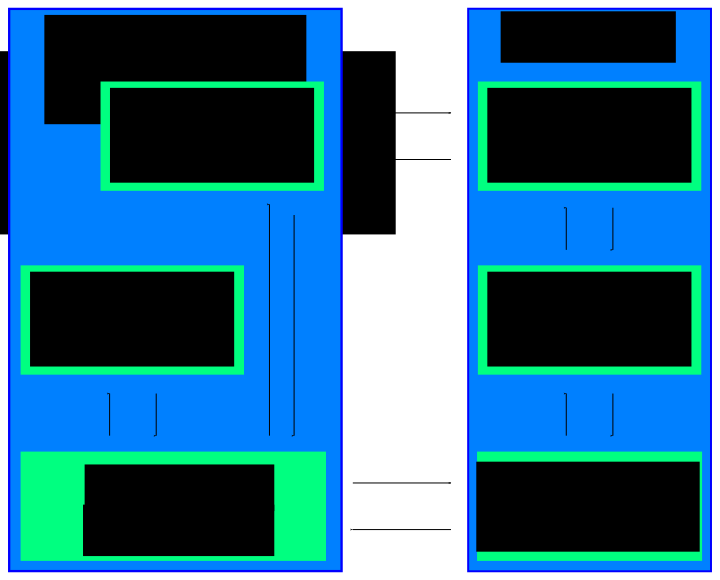
\includegraphics[height=0.75\paperheight,keepaspectratio]{system-full.png}
  \end{center}
\end{frame}

%---Current State Image Slide---%
\begin{frame}[c]{Current State}
  \begin{center}
    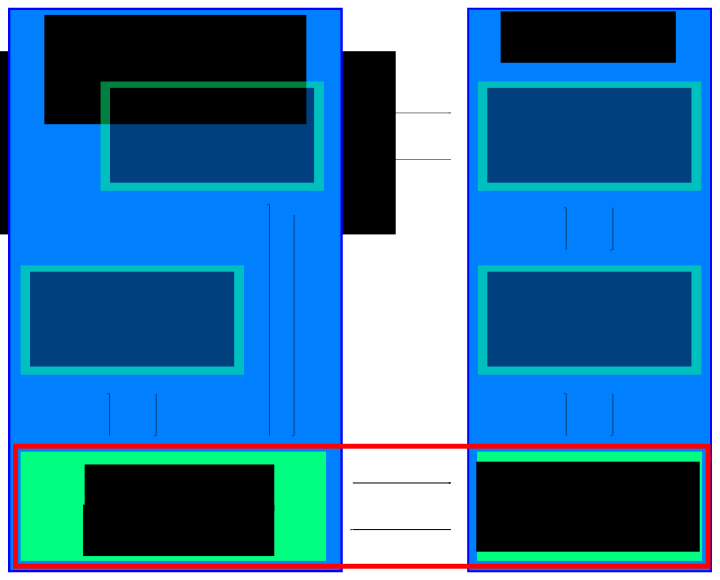
\includegraphics[height=0.75\paperheight,keepaspectratio]{system-working.png}
  \end{center}
\end{frame}

%---Current State Slide---%
\begin{frame}{\bf Current State}

\begin{itemize}
\item Supports exporting a single character device from the server
\item Supports importing a single character device on the client
\item Supports open, close, read, and write calls
\item Supports basic Linux udev operation for automatic node
  creation on client
\item Tested with various ``real'' and device files
\end{itemize}

\end{frame}

%---ToDo Slide---%
\begin{frame}{\bf ToDo}

\begin{itemize}
\item Multi-device, multi-server client-side import support
\item Multi-device server-side export support
\item Support for exclusive use and protection of exported devices
\item Support for ioctl calls
\item Support for providing and obtaining metadata for exported
  devices
\item Support for ``advertisement'' of available exported devices
\item Support for integrating imported devices into other kernel
  subsystems (human interface subsystem, audio subsystem, etc)
\item Addition of ``NCD-admin'' utilities for managing and administering
  NCD system
\item Addition of graceful connect and disconnect handling in real-time
\end{itemize}

\end{frame}

%---Advantages Slide---%
\begin{frame}{\bf Advantages}

What are the benefits of using Networked Character Device?

\begin{itemize}
\item Divorces peripherals from the computers to which they are
  attached
\item Allows simple creation of a ``Device Server''
\item Extends the ``Everything Is A File'' -nix Philosophy
\item Allows more efficient use of devices
\item Allows devices to be networked in a generalized, uniform manner
\end{itemize}

\end{frame}

%---Challenges Slide---%
\begin{frame}{\bf Challenges}

But there are difficulties making it work on a production scale...

\begin{itemize}
\item Does not work well when Character Device is not the exclusive
  device interface
  \begin{itemize}
  \item Many modern day devices interface directly with other
    in-kernel function, interfaces, and APIs
  \item procfs and sysfs provide additional device interface points
  \item Socket interfaces (netlink, etc) provide alternative to file
    system interfaces
  \end{itemize}
\item Requires exported devices to be ``de-integrated'' from host system
\item Requires QOS guarantees and high guilty network connection
\end{itemize}

\end{frame}

%---Potential Uses Slide---%
\begin{frame}{\bf Potential Uses}

What can we use NCDs for?

\begin{itemize}
\item Quick, cheap, and simple ad-hoc network KVM systems
\item Remote, networked web-cams, scanners, printers, etc
\item Basis of ``protocol''-over-Ethernet systems (USB-over-Ethernet,
  SATA-over-Ethernet, Etc)
\item Basis of redundant, ``cloud-like'' device pools
\item Basis of peripheral cluster systems (GPU Clusters, RNG Clusters,
  Etc)
\end{itemize}

\end{frame}


\section{Future Work}
%---Potential Uses Slide---%
\begin{frame}{\bf Future Work}

\begin{itemize}
\item Add multi-device, multi-server support
\item Add kernel sub-system handler layer (HID, etc)
\item Add device protection and removal capabilities to server system
\item Add advertisement protocol
\item Consider removing networking code from client kernel module
\end{itemize}

\end{frame}

\section{Conclusion}

\section{Bibliography}
%---Bibliography---%
\begin{frame}{\bf Bibliography}

\bibliography{refs}

\end{frame}

\end{document}

% vim: set sw=2 ts=2 et : %
